%Dokumentenklasse "scrbook" - Erweitert um den Verweis auf die Verzeichnisse und Texteigenschaften
\documentclass[chapterprefix=true, 12pt, a4paper, oneside, parskip=half, listof=totoc, bibliography=totoc, numbers=noendperiod]{scrbook}

% Ränder (Standard bottom ca. 52mm anbzüglich von ca. 4mm für die nach oben rechts gewanderte Seitenzahl)
%Anpassung der Seitenränder
\usepackage[bottom=48mm,left=25mm,right=25mm]{geometry}

% Ränder bei Bedarf zeigen
%\usepackage{showframe}

%Tweaks für scrbook
\usepackage{scrhack}

%Blindtext
\usepackage{blindtext}

%Erlaubt unteranderem Umbrücke captions
\usepackage{caption}

%Stichwortverzeichnis
\usepackage{imakeidx}

%Kompakte Listen
\usepackage{paralist}

%Zitate besser formatieren und darstellen
\usepackage{epigraph}

%Glossar, Stichworverzeichnis
\usepackage[toc, acronym]{glossaries} % Akronyme werden als eigene Liste aufgeführt
\usepackage{acronym}
%Anpassung von Kopf- und Fußzeile
%beinflusst die erste Seite des Kapitels
\usepackage[automark,headsepline]{scrlayer-scrpage}
\automark{chapter}
\ihead{\leftmark}
\chead{}
\ohead{\thepage}
\ifoot*{}
\cfoot[\thepage]{}
\cfoot*{}
\ofoot*{}
\pagestyle{scrheadings}

%Auskommentieren für die Verkleinerung des vertikalen Abstandes eines neuen Kapitels
%\renewcommand*{\chapterheadstartvskip}{\vspace*{.25\baselineskip}}

%Zeilenabstand 1,5
\usepackage[onehalfspacing]{setspace}

%Verbesserte Darstellung der Buchstaben zueinander
\usepackage[stretch=10]{microtype}

%Deutsche Bezeichnungen für angezeigte Namen (z.B. Innhaltsverzeichnis etc.)
\usepackage[ngerman]{babel}

%Unterstützung von Umlauten und anderen Sonderzeichen (UTF-8)
\usepackage{lmodern}
\usepackage[utf8]{luainputenc}
\usepackage[T1]{fontenc}

%Einfachere Zitate
\usepackage{epigraph}

%Verwendung von Akronymen
\usepackage[printonlyused]{acronym}

%Unterstützung der H positionierung (keine automatische Verschiebung eingefügter Elemente)
\usepackage{float} 

%Erlaubt Umbrüche innerhalb von Tabellen
\usepackage{tabularx}

%Erlaubt Seitenumbrüche mit Tabellen
\usepackage{longtable}

%Erlaubt die Darstellung von Sourcecode mit Highlighting
\usepackage{listings}

%Definierung eigener Farben bei nutzung eines selbst vergebene Namens
\usepackage[table,xcdraw]{xcolor}

%Vektorgrafiken
\usepackage{tikz}

%Grafiken (wie jpg, png, etc.)
\usepackage{graphicx}

%Grafiken von Text umlaufen lassen
\usepackage{wrapfig}

%Ermöglicht Verknüpfungen innerhalb des Dokumentes (e.g. for PDF), Links werden durch "hidelink" nicht explizit hervorgehoben
\usepackage[hidelinks,german]{hyperref}

%Einbindung und Verwaltung von Literaturverzeichnissen
\usepackage{csquotes} %wird von biber benötigt
\usepackage[style=alphabetic, backend=biber, bibencoding=ascii]{biblatex}
\addbibresource{references/references.bib}

%-------------------------------Zusätzliche Anpassungen und Modifikationen--------------------------------------------%

%Anpassung der Überschriften
\addtokomafont{disposition}{\rmfamily}

%Zusätzliche Farben
\definecolor{darkgreen}{RGB}{0,100,0}

%Umbenennungen
\renewcommand{\lstlistlistingname}{Quelltextverzeichnis}

%Pluszeichen in der Referenc beim zitieren ausblenden
\renewcommand*{\labelalphaothers}{}

%Anpassugen zur Quelltextdarstellung, kann bei Bedarf überschrieben werden (z.B. wenn unterschiedliche Sprachen zum Einsatz kommen)
\renewcommand{\lstlistingname}{Codeauszug}
\lstset{
	language=Java,
	numbers=left,
	columns=fullflexible,
	aboveskip=5pt,
	belowskip=10pt,
	basicstyle=\small\ttfamily,
	backgroundcolor=\color{black!5},
	commentstyle=\color{darkgreen},
	keywordstyle=\color{blue},
	stringstyle=\color{gray},
	showspaces=false,
	showstringspaces=false,
	showtabs=false,
	xleftmargin=16pt,
	xrightmargin=0pt,
	framesep=5pt,
	framerule=3pt,
	frame=leftline,
	rulecolor=\color{green},
	tabsize=2,
	breaklines=true,
	breakatwhitespace=true,
	prebreak={\mbox{$\hookleftarrow$}}
}

%Anpassungen für das Abkürzungsverzeichnis
\newglossarystyle{dottedlocations}{%
	\glossarystyle{list}%
	\renewcommand*{\glossaryentryfield}[5]{%
		\item[\glsentryitem{##1}\glstarget{##1}{##2}] \emph{##3}%
		\unskip\leaders\hbox to 2.9mm{\hss.}\hfill##5}%
	\renewcommand*{\glsgroupskip}{}%
}

\newcommand{\sieheKapitel}[1]{\glqq {#1}\grqq}
\newcommand{\sieheAbbVerweis}[2]{(siehe Abb. {#1} -- {#2})}
\newcommand{\sieheAbb}[1]{(siehe Abb. {#1})}
\newcommand{\sieheCA}[1]{(siehe Codeauszug {#1})}

\usepackage{chngcntr}
\counterwithout{footnote}{chapter}
%%Titles - Uncomment one section of titles
\usepackage[format=plain, justification=RaggedRight, singlelinecheck=false]{caption}
%%Used for titleGraduation
\makeatletter

\newcommand*{\logoPathL}[1]{\gdef\@logoPathL{#1}}
\newcommand*{\logoWidthL}[1]{\gdef\@logoWidthL{#1}}
\newcommand*{\logoPathR}[1]{\gdef\@logoPathR{#1}}
\newcommand*{\logoWidthR}[1]{\gdef\@logoWidthR{#1}}
\newcommand*{\gradeType}[1]{\gdef\@gradeType{#1}}
\newcommand*{\firstExaminer}[1]{\gdef\@firstExaminer{#1}}
\newcommand*{\secondExaminer}[1]{\gdef\@secondExaminer{#1}}
\newcommand*{\matrikelnr}[1]{\gdef\@matrikelnr{#1}}
\newcommand*{\submitDate}[1]{\gdef\@submitDate{#1}}

\renewcommand*{\maketitle}{
	\begin{titlepage}
		\newgeometry{left=2.5cm,right=2.5cm,top=3.0cm,bottom=2.5cm}
		\begin{center}
			\begin{figure}[h]
				\begin{minipage}[hbt]{6cm}
					\flushleft
					\ifx\@logoPathL\empty
					\else
					\includegraphics[width=\@logoWidthL\textwidth]{\@logoPathL}
					\fi
				\end{minipage}
				\hfill
				\begin{minipage}[hbt]{6cm}
					\flushright
					\ifx\@logoPathR\empty
					\else
					\includegraphics[width=\@logoWidthR\textwidth]{\@logoPathR}
					\fi
				\end{minipage}
			\end{figure}
			\vfill
			{\Large \@title\par}
			\vskip 0.5cm
			{\large \bfseries Projektbericht\par}
			\vskip 0.5cm
			{\large \textbf{Studiengang:}\\ 
			Internationale Medieninformatik}
			\vskip 0.5cm
			{\large \textbf{Betreuer:}\\ 
			Prof. Dr.-Ing. Carsten Busch / Alexander Kramer}
			\vskip 0.5cm
			{\large \textbf{Autor:}\\
			Chris Wodäge\\Matrikelnummer: 560597}
			\vskip 2cm
			{Independent coursework \\ Sommersemester 2018}
			\vfill
			\begin{flushleft}
				\begin{tabular}[t]{rl}
					
				\end{tabular}
			\end{flushleft}
		\end{center}
		\restoregeometry
	\end{titlepage}
}
\makeatother
\logoPathL{} %just leave empty to hide logo
\logoWidthL{0.5}
\logoPathR{resources/1000px-Logo_HTW_Berlin.png} %just leave empty to hide logo
\logoWidthR{1}
\gradeType{}
\secondExaminer{}

%%Used for titleResearchPaper
%\makeatletter

\newcommand*{\firstExaminer}[1]{\gdef\@firstExaminer{#1}}
\newcommand*{\subTitle}[1]{\gdef\@subTitle{#1}}
\newcommand*{\researchPart}[1]{\gdef\@researchPart{#1}}
\newcommand*{\matrikelnr}[1]{\gdef\@matrikelnr{#1}}
\newcommand*{\submitDate}[1]{\gdef\@submitDate{#1}}


\renewcommand*{\maketitle}{
	\begin{titlepage}
		\newgeometry{left=2.5cm,right=2.5cm,top=9.0cm,bottom=2.5cm}
		\begin{center}
			\vfill
			{\Large \@title\par}
			{\normalsize \@subTitle\par}
			\vskip 0.5cm
			{\large \bfseries Forschungsprojekt Teil \@researchPart\par}
			\vskip 0.5cm
			{\large an der}
			\vskip 0.5cm
			{\large Hochschule für Technik und Wirtschaft Berlin\\ Fachbereich 4 - Informatik, Kommunikation und Wirtschaft\\ Studiengang Angewandte Informatik}
			\vfill
			\begin{flushleft}
				\begin{tabular}[t]{rl}
					Betreuer: &\@firstExaminer\\
					\\
					Eingereicht von: &\@author\\
					\ifx\@matrikelnr\empty
					\else
					Matrikelnummer: & \@matrikelnr\\
					\fi
					Datum der Abgabe: & \@submitDate
				\end{tabular}
			\end{flushleft}
		\end{center}
		\restoregeometry
	\end{titlepage}
}
\makeatother
%\subTitle{Ein optionaler Untertitel der Arbeit}
%\researchPart{A}

%%Used by all titles
\title{IndustrialVR -- Erstellung einer Virtual Reality Anwendung mit Unity auf Basis von 3D-CAD Daten.}
\author{Chris Wodäge}
\matrikelnr{s0560597} % just leave empty to hide number
\submitDate{05.10.2015}
\firstExaminer{Max Mustermann}
%%End Titles

\makeindex[title=Stichwortverzeichnis, options=-s indexstyle.ist, intoc]
\indexsetup{level=\chapter*,toclevel=chapter}

\makeglossaries
\loadglsentries{glossary_and_acronyms.tex}
\setacronymstyle{long-short}

\begin{document}

\pagenumbering{alph} %fix for same identifier warning, character is not show in title
\maketitle



% Eigenständigkeitserklärung / Abkürzvz
\null\thispagestyle{empty}
\pagenumbering{Roman}
\addchap{Eigenständigkeitserklärung}

Hiermit versichere ich, dass ich die vorliegende Arbeit selbstständig und nur unter
Verwendung der angegebenen Quellen und Hilfsmittel verfasst habe. Die Arbeit wurde bisher
in gleicher oder ähnlicher Form keiner anderen Prüfungsbehörde vorgelegt.

\vskip 1cm

Berlin, den 28.09.2018

\vskip 1.5cm

Chris Wodäge
\input{chapter/Abkürzungsverzeichnis} 

%Abbildungen
\listoffigures \clearpage
\tableofcontents \newpage


\pagenumbering{arabic}


%%============== Neue Seiten ============== %%
\input{chapter/1Einführung} \clearpage
\chapter{Datenverarbeitung in CAD}
\section{Anwendungsbereiche von CAD}
\label{sec:DatenverarbeitungInCAD}

Die Grundlage dieser Arbeit sowie des Prototypen bilden Daten, welche in 3D-CAD-Programmen erstellt wurden. Daher wird im Rahmen dieser Arbeit CAD als Synonym für 3D-CAD verwendet. Im Gegensatz zu 2D-CAD Systemen können in 3D-CAD Systemen Produkte realer konstruiert werden. Das kann sich positiv auf die Entwicklungszeit auswirken. Kollisionsbetrachtungen ermöglichen eine Fehlererkennung, bevor das erste Teil gefertigt wird.\footnote{Vgl. Dipl. Ing. (FH) Bettina Clauß, Helmut Prof. Dr.-Ing. von Eiff (2013): \textit{CAD Grundkurs}. Hochschule Esslingen, S. 2.} Es ist möglich in CAD anhand von Materialeigenschaften physikalische Eigenschaften wie z.B. Festigkeit, Elastizität etc. zu simulieren. Aufgrund dieser Flexibilität sind CAD-Programme heute in fast allen technischen Zweigen vertreten, darunter Architektur, Bauingenieurwesen, Maschinenbau, Elektrotechnik bis hin zur Zahntechnik.\footnote{Vgl. Wikipedia  (2018): \textit{CAD}.\newline
\url{https://de.wikipedia.org/w/index.php?title=CAD&oldid=178934444},\newline 
abgerufen am 23.08.2018.}


\section{3D-Modellierung in CAD}
\label{sec:3D-ModellierungInCAD}
In CAD werden Modelle in dreidimensionaler Form modelliert und persistiert. Ein dreidimensionaler Aufbau ermöglicht das Nachbilden einer realitätsnahen Darstellung, das Rendern aus allen Blickwinkeln und Perspektiven sowie eine bessere räumliche Betrachtung. Das Hauptaugenmerk des Ingenieurs liegt dabei vor allem auf Funktionalitäten wie dem technischen Zeichnen, der Erstellung von Arbeitsplänen, Montage- und Bedienungsanleitungen. Weitere Anforderungen sind unter anderem technisch visuelle Darstellungen, wie die Kollisionsbetrachtung oder die Zusammenbau-, Einbau- und die Montageuntersuchung.
Die in dieser Arbeit thematisierte Betrachtung bezieht sich vor allem auf die Nutzung außerhalb der CAD-Umgebung.  Der Vollständigkeit halber werden nachfolgend alle drei recheninternen Repräsentationen, die in CAD vorliegen betrachtet.

\begin{itemize}
\item \textbf{Kantenmodelle:} Kantenmodelle (auch Drahtgitter oder Wireframe) repräsentieren ein Objekt anhand von Kanten. Diese Darstellung enthält keinerlei Informationen über die Flächen oder das Volumen eines Körpers. Kantenmodelle dienen häufig als Hilfsgeometrie zur Erzeugung von Flächen oder als Darstellungsart von Volumen- oder Flächenmodellen.

\item \textbf{Flächenmodelle:} Als Flächenmodelle werden \glqq hohle\grqq\ Objekte bezeichnet, deren äußere Form durch Flächen beschrieben wird. Eine intuitive Anpassung der Objekthülle ist mit Hilfe von Kontrollpunkten oder Kontrollnetzen ohne Einschränkung möglich. Unter Zuhilfenahme von analytisch beschreibbarer (Translationsflächen, Regelflächen) sowie analytisch nicht beschreibbarer Flächen (B-spline-, NURBS-Flächen) lassen sich jegliche Formen modellieren.

\item \textbf{Volumenmodelle:} Unter Volumenmodellen versteht man Körper, die neben einer Hülle auch eine Materialdichte besitzen, woraus das CAD-System  automatisch eine Masse interpretiert. Auf diese Weise bleibt die geometrische Konsistenz bei Manipulation des Objektes erhalten. Aufgrund dieses zusätzlichen Parameters kann ein hoher Grad an Automatisierung sichergestellt werden. Es können Eigenschaften wie Trägheit, Schwerpunkt, Gewicht etc. durch das CAD-System automatisch abgeleitet und als Parameter für Simulationen übergeben werden.  
\end{itemize}

Auf alle beschriebenen Modelle lassen sich räumliche Operationen wie Translation, Rotation und Skalierung anwenden. Zusätzlich existieren für jedes Modell spezielle Werkzeuge um diese zu verformen, zu zerschneiden, zu verdrehen oder anderweitig zu manipulieren.\footnote{Vgl. Wikipedia  (2018): \textit{CAD}.\newline
\url{https://de.wikipedia.org/w/index.php?title=CAD&oldid=178934444},\newline 
abgerufen am 23.08.2018.} 

\section{Exportformat in CAD}
\label{sec:ExportformatInCAD}

Für den Export aus SolidWorks einem 3D-CAD-Programm des französischen Softwareentwicklers Dassault Systèmes musste ein Dateiformat gefunden werden, dass auch von einem gängigen 3D-Programm geparsed werden kann. Als alternivlos hat sich das Dateiformat \glqq STL\grqq\, erwiesen. Das Ergebnis des Exportes war nicht optimal (siehe \sieheKapitel{\hyperref[sec:AnalyseDesCAD-Exports]{3.2 Analyse des CAD-Exports}}). Nichtsdestotrotz hat die Übertragung schnell und ohne essentiellen Informationsverlust funktioniert.
STL -- Standard Transformation Language,  Surface Tessellation Language oder Standard Triangulation Language ist einer der ältesten und im Kontext des 3D-Druckes das gängigste Format.  
STL beschreibt die Oberfläche eines Objektes näherungsweise durch Triangulation mit unterschiedlich großen Dreiecken. Der Datensatz besteht aus den Koordinaten der Eckpunkte jedes Dreiecks sowie dessen Normalenvektor \sieheCA{2.1\footnote{Dave Touretzky (o.J.): \textit{STL Files and Slicing Software}. Carnegie Mellon University Pittsburgh, Pennsylvania, S. 5.}}.\footnote{Vgl. Heiko Heckner, Marco Wirth (2014): \textit{Vergleich von Dateiformaten für 3D-Modelle}. Julius-Maximilians-Universität Würzburg, S. 8.}


\begin{lstlisting}[caption={STL ASCII Schema.}, captionpos=b, label={lst:STL ASCII}]
solid <name>
facet normal ni nj nk
   outer loop
      vertex v1x v1y v1z
      vertex v2x v2y v2z
      vertex v3x v3y v3z
   endloop
endfacet
...
endsolid <name>

\end{lstlisting}

Da Autodesk Maya und andere (nicht CAD) 3D-Programme ausschließlich auf Basis von Flächenmodellen arbeiten, müssen keine weiteren Informationen bzgl. des Modells übertragen werden. \clearpage
\chapter{Aufbereitung der 3D-CAD Daten}
\label{sec:AufbereitungDer3D-CADDaten}

\section{Eine kurze Einführung zum Aufbau von 3D-Objekten}
\label{sec:KurzerEinschubZumAufbauVon3D-Objekten}

\begin{wrapfigure}{R}{0.5\textwidth}
	\centering
	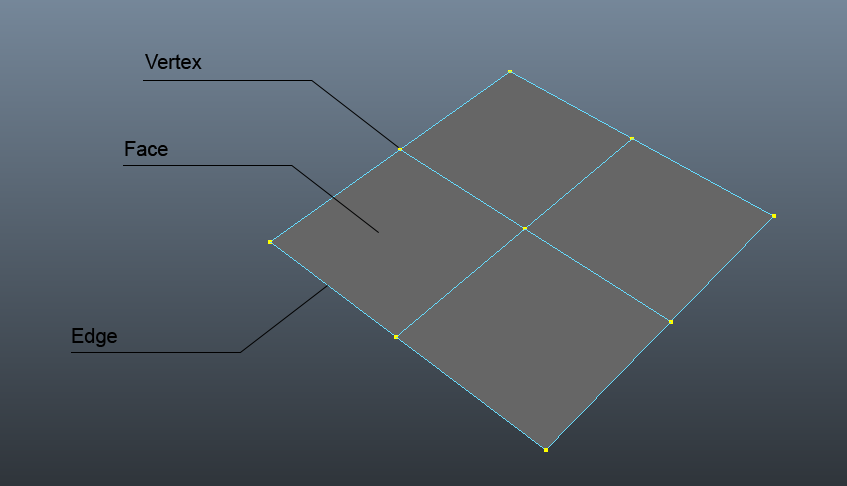
\includegraphics[width=0.5\textwidth]{bildquellen/face_edge_vertex}
	\caption{Eine Plane, bestehend aus vier quadratischen Polygonen.}
\end{wrapfigure}
In gängigen 3D-Programmen geschieht die Modellierung mit Hilfe von polygonalen Netzen (meshes), welche in der 3D-Computergrafik häufig anzutreffen sind. Polygonnetze, also Netze die sich aus einer Menge von miteinander verbundenen Polygonen zusammensetzen, bestehen zumeist aus Dreiecken und Vierecken. Es lassen somit einfache geometrische Figuren wie Zylinder, Kugeln, Prismen, Würfel, Tetraeder, Pyramiden etc. aber auch komplexere Strukturen erschaffen, um bspw. Modelle für Computerspiele oder Animationsfilme zu erstellen.\footnote{Vgl. Michael Bender, Manfred Brill (2006): \textit{Computergrafik}. 2.Aufl. München: \newline Carl Hanser Verlag. S. 19.}

In Autodesk Maya werden polygonale Flächen auch als Faces bezeichnet und haben drei oder mehr begrenzende Kanten, die Edges genannt werden. Die Edges wiederum sind über Punkte, den sogenannten Vertices (Plural) miteinander verbunden. Diese drei formgebenden Elemente können transformiert werden, um ein polygonales Netz zu deformieren. Genutzt werden dafür die verschiedenen Transform-Attribute, Translation, Rotation und Skalierung.\footnote{Vgl. Todd Palamer (2014): \textit{Vgl. Mastering Autodesk Maya 2015}. 1.Aufl. Indianapolis: Sybex. S. 107 f.} Zusätzlich können weitere Unterteilungen eingesetzt werden, um ein Polygonnetz feiner zu strukturieren. Es ist möglich Faces, Edges und Vertices miteinander zu verbinden, aufzutrennen oder um jeweils neue Elemente zu erweitern (extrudieren). 

\section{Analyse des CAD-Exports}
\label{sec:AnalyseDesCAD-Exports}
Bevor das aus CAD exportierte Modell in Unity importiert wird sollte selbiges vorher in einem geeigneten 3D-Programm überprüft werden. Für diesen Zweck wird, wie im vorangegangenen Kapitel erwähnt auf Autodesk Maya zurückgegriffen. Maya ist eine professionelle Software für Modellierung, Animation und Rendering von 3D Objekten und Szenen.\footnote{Vgl. Autodesk  (2018): \textit{MAYA}.\newline
\url{https://www.autodesk.de/products/maya/overview},\newline 
abgerufen am 30.08.2018.}

\begin{figure}[H]
	\centering
	\captionsetup{width=1\textwidth}
	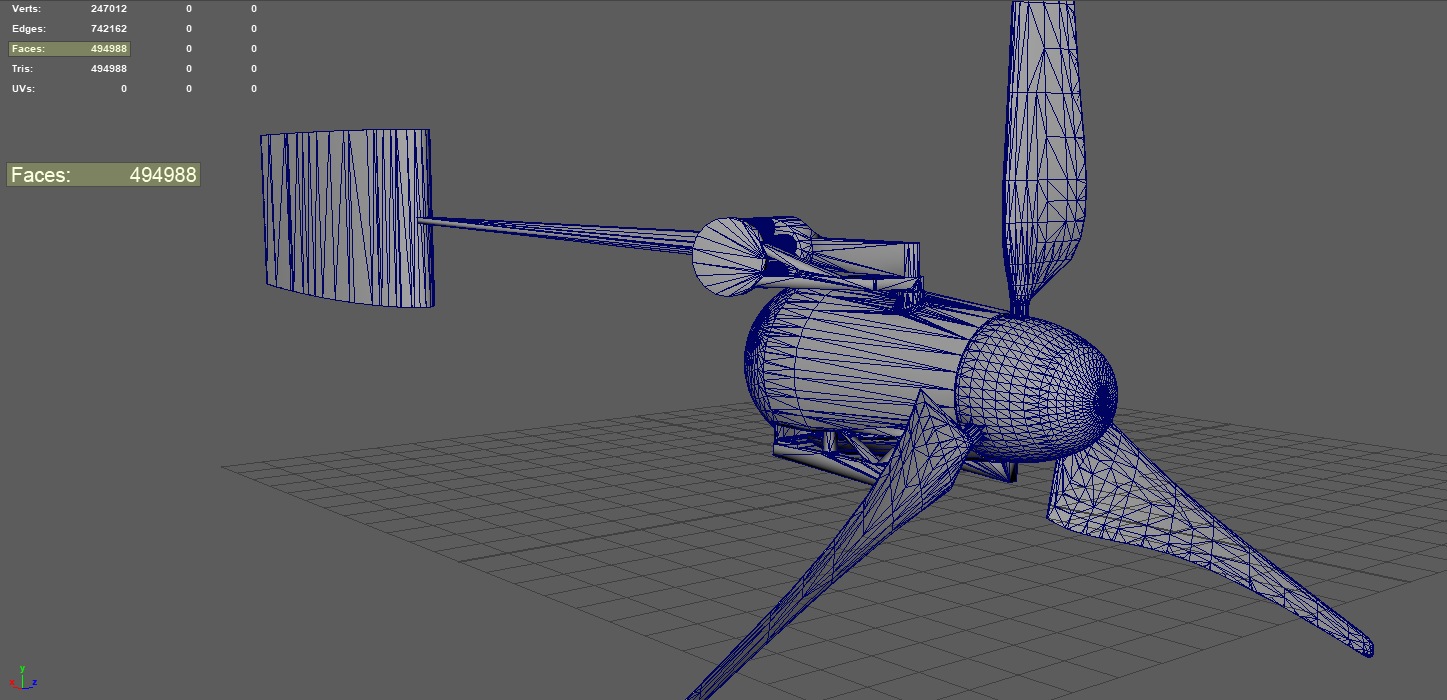
\includegraphics[keepaspectratio, width=1\textwidth]{bildquellen/WEA-Vergleich1}
	\caption{Ergebnis des Exportes der WEA aus der CAD-Anwendung bestehend aus 494.988 Polygonen.}
	\label{fig:2.2}
\end{figure}

Das importierte Modell \sieheAbb{2.1} weist mehrere Eigenschaften auf, welche es für einen Import sowie eine Weiterverarbeitung in Unity ungeeignet machen. Die betreffenden Eigenschaften sind nachfolgend aufgelistet. 
Generell sollten Modelle mit möglichst wenigen Polygonen auskommen, da ein hoher Detailgrad über Texturen generiert werden kann. Im Falle einer technischen Darstellung die neben der äußeren Verkleidung auch innenliegende technische Baugruppen wie Wälzlager, Getriebe o.ä. abbildet, kann dass die Anzahl der Polygone deutlich erhöhen. Schließlich müssen diese in adäquater Qualität dargestellt werden. Natürlich gilt aber auch hier der Grundsatz, dass eine zu geringe Anzahl zu lasten der Darstellungsqualität und eine zu hohe Anzahl zu lasten der Performance geht. Es gilt also einen guten Mittelweg zu finden. 


\begin{itemize}
\item \textbf{Polygon count:} Das Modell besteht aus nicht ganz 500.000 Polygonen, was für eine Echtzeitanwendung sehr viel ist. Laut der Unity Dokumentation sollte der Polycount von dem Zielsystem und der angestrebten Qualität abhängig sein. Das Optimum liegt für Desktopanwendungen bei 1500 bis 4000 Polygonen pro Objekt. Falls sehr viele Objekte zur selben Zeit aktiv sind wird eine Reduktion der Polygone empfohlen.\footnote{Vgl. Unity Documentation  (2018): \textit{Modeling characters for optimal performance}.\newline
\url{https://docs.unity3d.com/Manual/ModelingOptimizedCharacters.html},\newline 
abgerufen am 30.08.2018.}     

\item \textbf{Unterteilung in Einzelobjekte:} Die WEA setzt sich aus vielen Einzelobjekten zusammen. Diese sind vom großen Rotorblatt bis zur kleinsten Schraube zu einem einzigen Objekt zusammengefasst. Es ist also nicht möglich einzelne Teilobjekte in Unity separat mit Materialien und Skripten auszustatten oder zu Animieren.  

\item \textbf{Flächenverteilung:} Ferner führt die ungleichmäßige Flächenverteilung im STL Export zu Darstellungsfehlern beim Shading \sieheAbb{2.2}. Eng zusammenliegende Edges beeinflussen das visuelle Endergebnis negativ.
\end{itemize}

\begin{figure}[H]
	\centering
	\captionsetup{width=1\textwidth}
	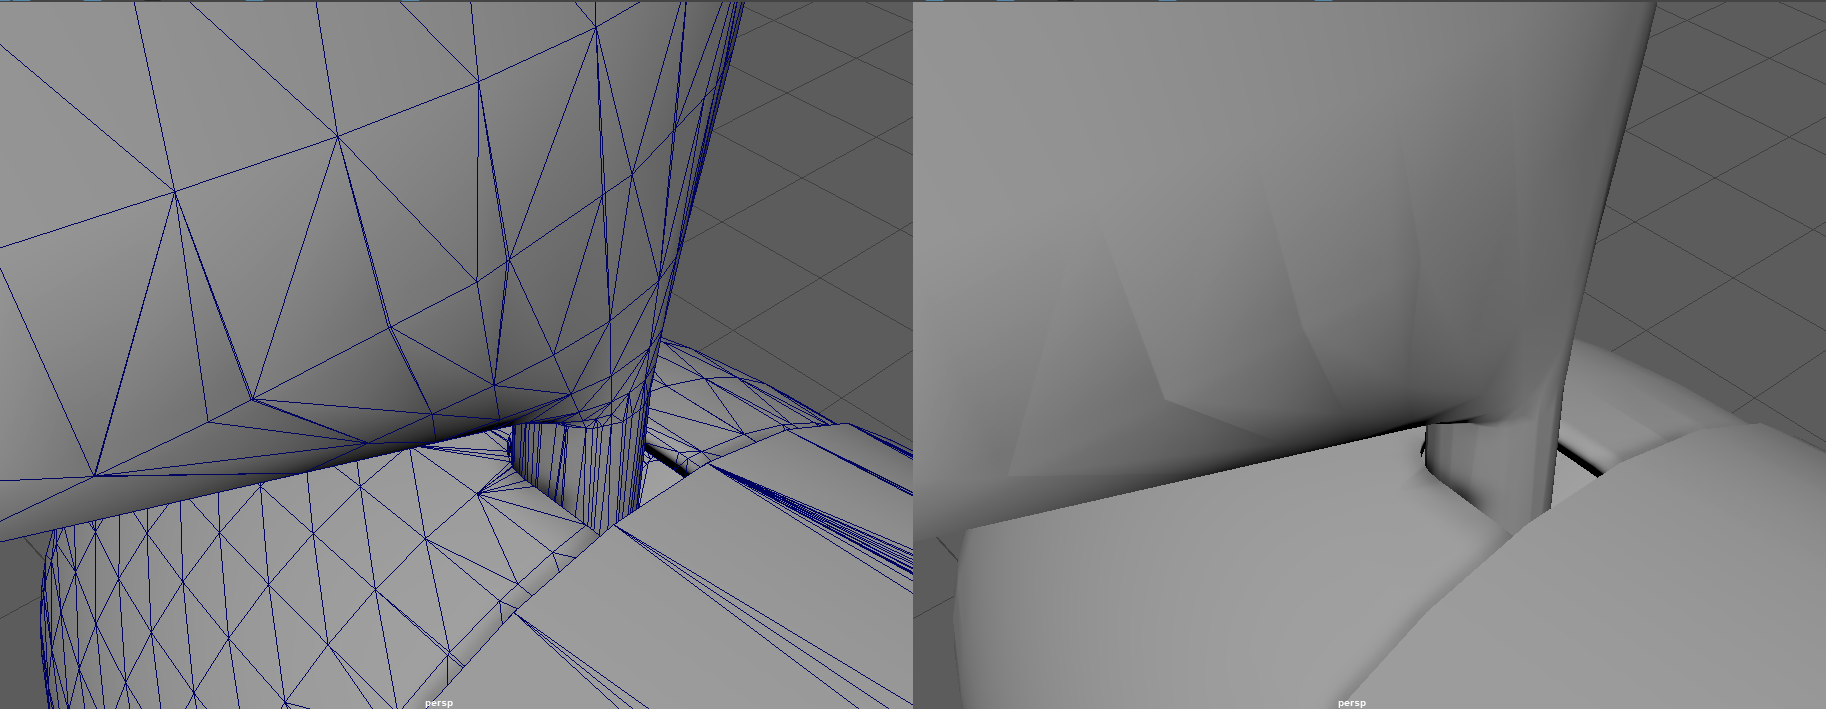
\includegraphics[keepaspectratio, width=1\textwidth]{bildquellen/WEAfehlerhaftesshading}
	\caption{Shadingfehler am Exportmodell.}
	\label{fig:2.3}
\end{figure}

Um diese Probleme zu lösen ist eine Retopologisierung also eine Überarbeitung der geometrischen Grundstruktur und eine damit einhergehende Reduktion der Flächen nötig. Diese Vorgehensweise wird im folgenden Kapitel \sieheKapitel{\hyperref[sec:RetopologisierungDesCAD-Exports]{3.3 Retopologisierung des CAD-Exports}} beschrieben.

\label{sec:RetopologisierungDesCAD-Exports}
\section{Retopologisierung des CAD-Exports}
Die Aufbereitung des Modells kann händisch oder automatisiert erfolgen. Die hänsiche Retopologisierung ist aufwändiger und erfordert Kenntnisse in der Polygonmodellierung. Die Qualität und die Anzahl der Polygone des Modells können aber exakt gesteuert werden. Eine automatische Reduktion hat aufgrund von invalider Geometrie, sogenannter non-manifold geometry aber nicht funktioniert. Das folgende Zitat aus der Maya LT Dokumentation von Autodesk beschreibt in Kürze das Problem. 

\begin{quote}
\glqq Some types of polygon geometry will not work in Maya. Invalid geometry includes vertices that are not associated with a polygon edge and polygon edges that are not part of a face (dangling edges). While Maya does not let you create these types of geometry, it may be possible to import these types from other software applications.\grqq\footnote{Autodesk  (2015): \textit{Two-manifold vs. non-manifold polygonal geometry}.\newline
\href{https://knowledge.autodesk.com/support/maya-lt/learn-explore/caas/CloudHelp/cloudhelp/2015/ENU/MayaLT/files/Polygons-overview-Twomanifold-vs--nonmanifold-polygonal-geometry-htm.html}{https://knowledge.autodesk.com/support/maya-lt/\dots},\newline abgerufen am 05.09.2018.} 
\end{quote}

Der Import aus CAD enthielt diese invalide Geometrie. Bei einem solch komplexen Modell eine Fehlersuche einzuleiten ist daher sehr zeitaufwendig werden und das Ergibnis der Autoreduktion ist Qualitativ minderwertiger wie die folgende Abbildung aus einem anderen Projekt zeigt \sieheAbb{2.4}. 

\begin{figure}[H]
	\centering
	\captionsetup{width=0.8\textwidth}
	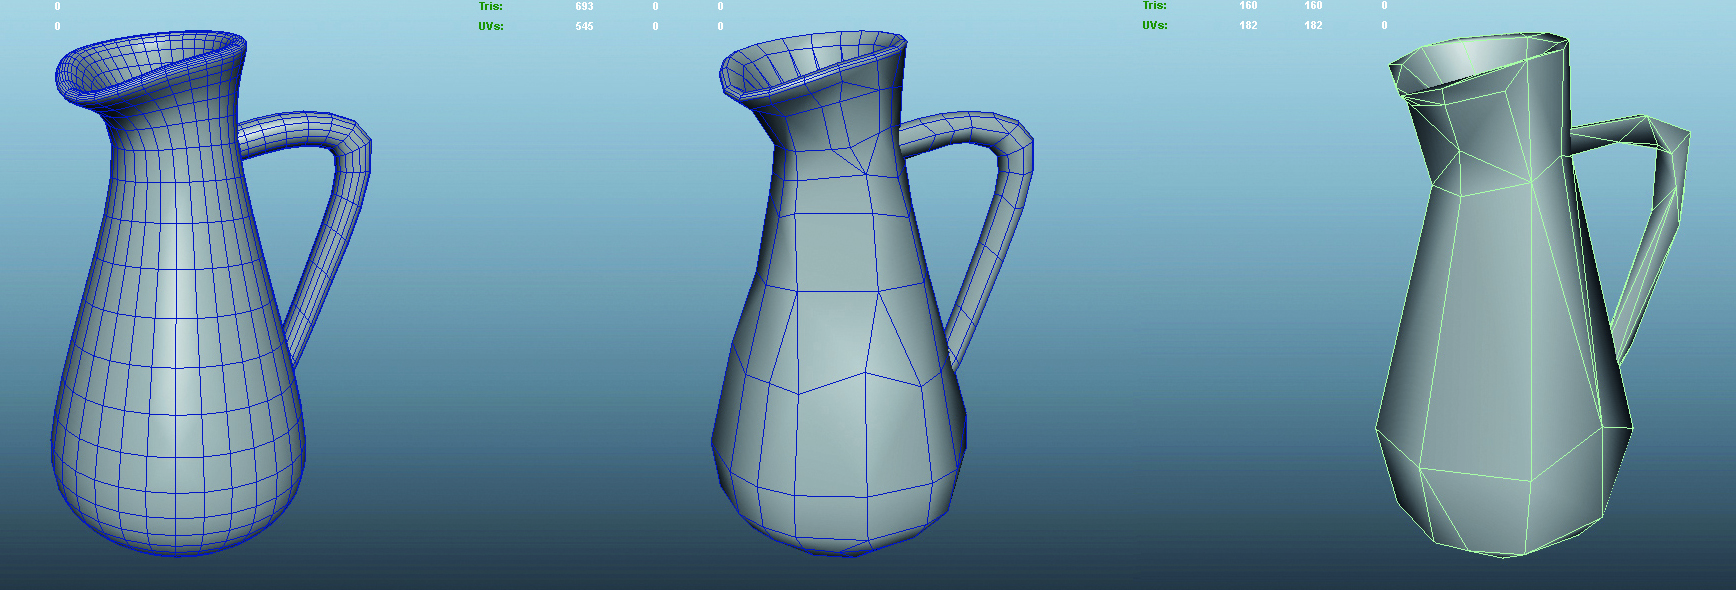
\includegraphics[keepaspectratio, width=0.8\textwidth]{bildquellen/hp-zu-lp-automatisch}
	\caption{Automatische Reduktion der Polygone auf (v.l.n.r.) 1536, 382 und 117.}
	\label{fig:2.4}
\end{figure}

Daher erschien es praktikabler das Modell händisch aufzubereiten. Die Aufbereitung erfolgte in Maya anhand von Polygonmodellierung auf Basis von primitiven Körpern (Primitives). das können bspw. Würfel, Cylinder, Kugeln, Tori etc. sein.  Mit Erzeugung dieser Primitives lässt sich durch Flächenextrusion die grobe Form nachbauen und mit Hilfe weiterer Unterteilungen verfeinern. Diese Anpassung des Primitives an die Form des CAD-Exportes geschieht für alle drei Raumdimensionen. Um eine sehr genaue Abbildung zu Erzeugen können die Vertices des erzeugten Primitives an die Vertices des CAD-Modells \glqq angedockt\grqq\, werden. Es ist mit wenigen Werkzeugen möglich eine Abbildung des ursprünglichen Objektes mit guter Topologie und einer deutlich reduzierten Anzahl an Polygonen zu erzeugen. Die Vorgehensweise wird nachfolgend anhand eines Beispiels verdeutlicht \sieheAbb{2.5}.

\begin{figure}[H]
	\centering
	\captionsetup{width=1\textwidth}
	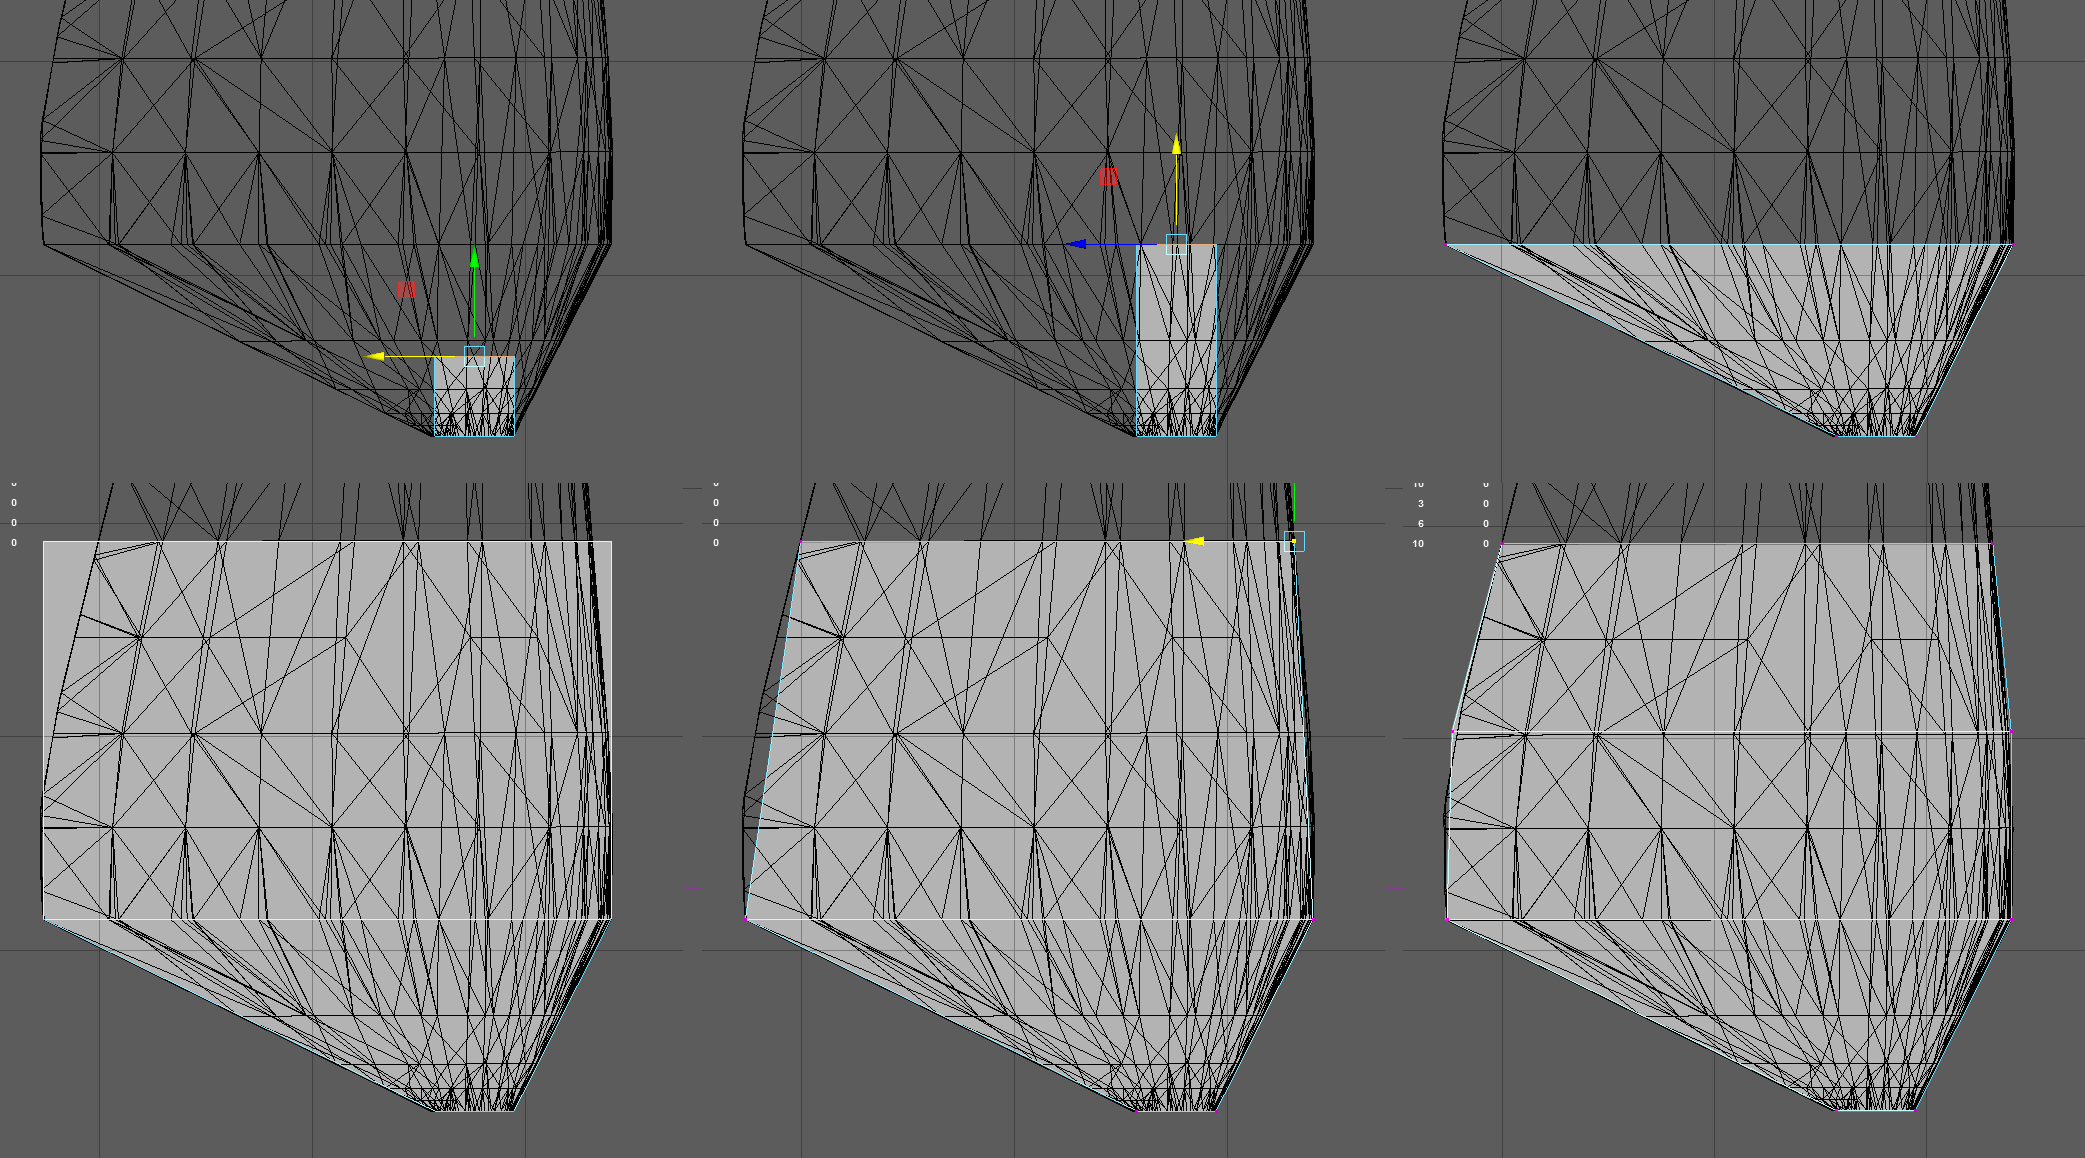
\includegraphics[keepaspectratio, width=1\textwidth]{bildquellen/mod}
	\caption{Retopologisierung einer Teilfläche durch Erzeugung eines Primitives, Anpassung der Vertices, Flächenextrusion und Einsetzen einer weiteren Unterteilung (Edgeloop).}
	\label{fig:2.5}
\end{figure}
 \clearpage
Die Gesamte Retopologisierung des CAD-Exportes fand mit mehr oder weniger diesen Werkzeugen statt. Die Abbildung verdeutlicht noch einmal den Unterschied. Das alte Rotorblatt weist eine Anzahl von 1130 Polygonen auf. Das neue Modell setzt sich aus 76 Polygonen zusammen. Es konnten also etwas mehr als 93\% der Flächen eingespart werden \sieheAbb{2.6}. 

\begin{figure}[H]
	\centering
	\captionsetup{width=1\textwidth}
	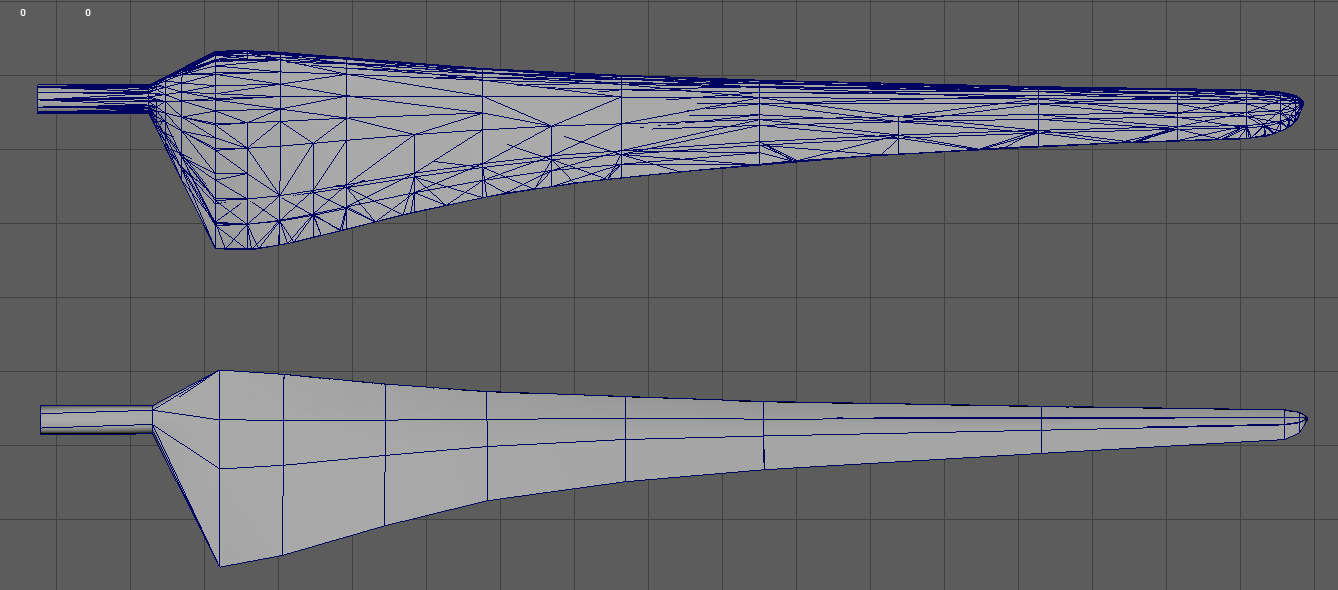
\includegraphics[keepaspectratio, width=1\textwidth]{bildquellen/rotorblattGeo}
	\caption{Vergleich des Rotorblattes aus dem CAD-Export (1130 Polygone) mit dem neu erstellten Rotorblatt(76 Polygone).}
	\label{fig:2.6}
\end{figure}

Für ein einzelnes Objekt sind über 1000 Polygone kein Problem. Da es sich bei diesem Rotorblatt aber um eines von vielen Bauteilen handelt, kann die Polygondichte sehr schnell ausufern und die Hardware überfordern. Wenn sich das Objekt mit weniger Polygonen ähnlich gut beschreiben lässt, sollte diese Sparmaßname unbedingt greifen. Zudem gilt natürlich auch hier der Grundsatz des sparsamen Umgangs mit Hardwareressourcen, wie dies generell in der Softwareentwicklung gewünscht wird.  

\begin{figure}[H]
	\centering
	\captionsetup{width=1\textwidth}
	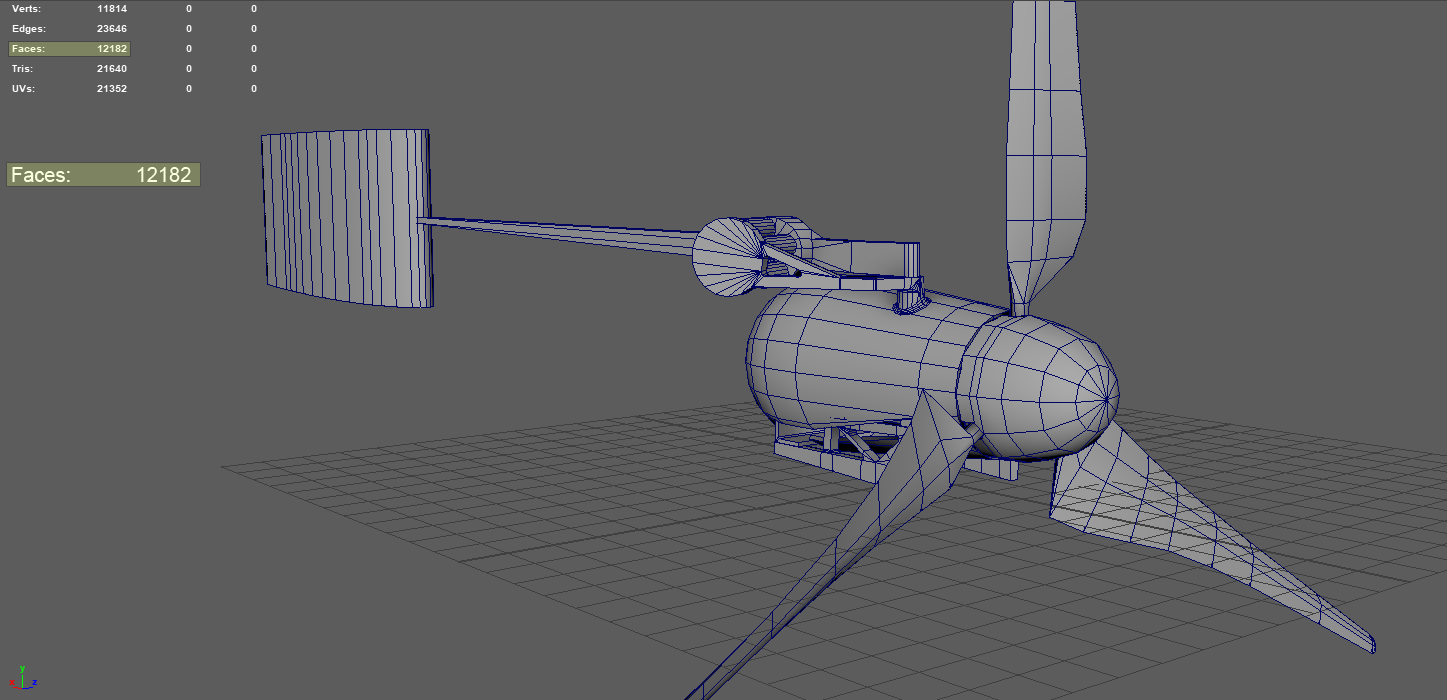
\includegraphics[keepaspectratio, width=1\textwidth]{bildquellen/WEA-Vergleich2}
	\caption{Ergebnis der Retopologisierung bestehend aus 12.182 Polygonen.}
	\label{fig:2.7}
\end{figure}

Das Endergebnis der Retopologisierung kann in der folgenden Abbildung betrachtet werden  \sieheAbb{2.7}. Im Gegensatz zum CAD-Export, der aus 494.988 Polygonen besteht, enthält das neue Modell nur 12.182 Polygone. Es lässt sich konstatieren, dass in Summe ca. 97,5 aller Flächen eingespart wurden.
 \clearpage
\chapter{Umsetzung in Unity}

\section{VRTK -- Virtual Reality Toolkit}
\label{sec:VRTK-VirtualRealityToolkit}

Für die Entwicklung des Prototypen wurde das  Virtual Reality Toolkit (VRTK) verwendet. VRTK ist ein Open-Source Framework für Unity mit dessen Hilfe es möglich ist, in kurzer Zeit eine voll funktionsfähige VR-Anwendung zu entwickeln. Das Projekt startete im April 2016 und wird seit dem weiterentwickelt.\footnote{Vgl. GitHub (2018): \textit{VRTK Code frequency}.\newline
\url{https://github.com/thestonefox/VRTK/graphs/code-frequency},\newline 
abgerufen am 06.09.2018.} 
Ein großer Vorteil des VRTK-Frameworks ist laut seinem Initiator Harvey Ball die Plattformunabhängigkeit. VRTK verfügt über eine Abstraktionsschicht die es ermöglicht, dass Komponenten für die Mechanik eines Spiels auf jedem unterstützen SDK funktionieren. Die Anwendung läuft auf SteamVR oder Oculus oder PSVR ohne zusätzlichen Programmieraufwand. Falls ein Projekt auf Basis von SteamVR entwickelt wird, man aber auf weitere Plattformen portieren möchte, so müssen Codeblöcke für andere SDKs umgeschrieben werden oder eben eine eigene Abstraktionsschicht entwickelt werden. Einige beliebte SteamVR Titel lassen sich laut Ball auch nicht ohne weiteres nach Oculus Home portieren. VRTK soll dieses Problem lösen.\footnote{Vgl. Ian Hamilton (2017): \textit{VRTK’s Open Source Tools Help New Developers Get Started In VR}.\newline
\url{https://uploadvr.com/vrtk-stone-fox-unity-tool/},\newline 
abgerufen am 06.09.2018.}
Unterstützt werden gängige VR-Platformen wie die Oculus Rift, Windows Mixed Reality oder die HTC VIVE. Auch eine Anbindung an Steam über das SteamVR Plugin ist möglich und wurde im Rahmen dieser Arbeit verwendet. Falls gerade keine VR-Hardware zur Verfügung steht, kann die Anwendung über den integrierten VR-Simulator getestet werden. 
Das VRTK-Framework implementiert die Grundlegenden Funktionalitäten, welche für eine VR-Anwendung benötigt werden. Dazu zählen unter anderem die Möglichkeit der Fortbewegung in einer Szene oder Interaktionen wie die Berührung, das Greifen und die Benutzung von Objekten.  Auch die Interaktion mit UI-Elementen durch Berührung oder mittels Pointer sind implementiert. Weiterhin ist die Benutzung von Kontrollelementen wie Buttons, Hebeln, Türen, Schubladen etc. möglich. Diese können, wenn nötig an gegebene Anforderungen angepasst.\footnote{Vgl. GitHub (2018): \textit{VRTK - Virtual Reality Toolkit}.\newline
\url{https://github.com/thestonefox/VRTK},\newline 
abgerufen am 05.09.2018.}

\section{Szenenaufbau in Unity}
\label{sec:Szenenaufbau}

Die Szene setzt sich aus verschiedenen Komponenten zusammen, die sich grob in drei Kategorien einteilen lassen.

\begin{itemize}
\item \textbf{Schaltpult:} Das \glqq Schaltpult zur Anlagensteuerung\grqq\,  \sieheAbbVerweis{4.1}{1} erfüllt verschiedene Funktionalitäten, welche die Steuerung der WEA betreffen. Weitere Erläuterungen sind im nachfolgenden Unterkapitel \sieheKapitel{\hyperref[sec:ImplementierteAnwendungsfälle]{4.3 Implementierte Anwendungsfälle}} beschrieben. 

\item \textbf{WEA:}  
Das eigentliche Modell der WEA  \sieheAbbVerweis{4.1}{2} ist in der Szene platziert. Anhand dieses Modells soll die Funktionsweise verdeutlicht werden. Aktuell sind vor allem Mechanische Komponenten implementiert und animiert. In weiteren Iterationen könnte bspw. das Thema Stromerzeugung mithilfe eines Generator in die Visualisierung mit einbezogen werden. 

\item \textbf{Hinweisschilder:} Die Hinweisschilder \sieheAbbVerweis{4.1}{3} dienen dazu, den Anwender über die Benennung der Komponenten zu informieren. Problematisch an dieser Darstellungsweise ist, dass zu viele Schilder auf einer zu kleinen Fläche sich gegenseitig überlagern können und dadurch die Lesbarkeit beeinträchtigt ist. Auch können diese andere Komponenten verdecken und so eine Betrachtung der WEA erschweren. Gerade an Stellen, an denen sich viele Komponenten auf kleinem Raum befinden ist dieses Problem aufgetreten. Daher können die Hinweisschilder jederzeit ausgeblendet werden.

\end{itemize}
  
\begin{figure}[H]
	\centering
	\captionsetup{width=1\textwidth}
	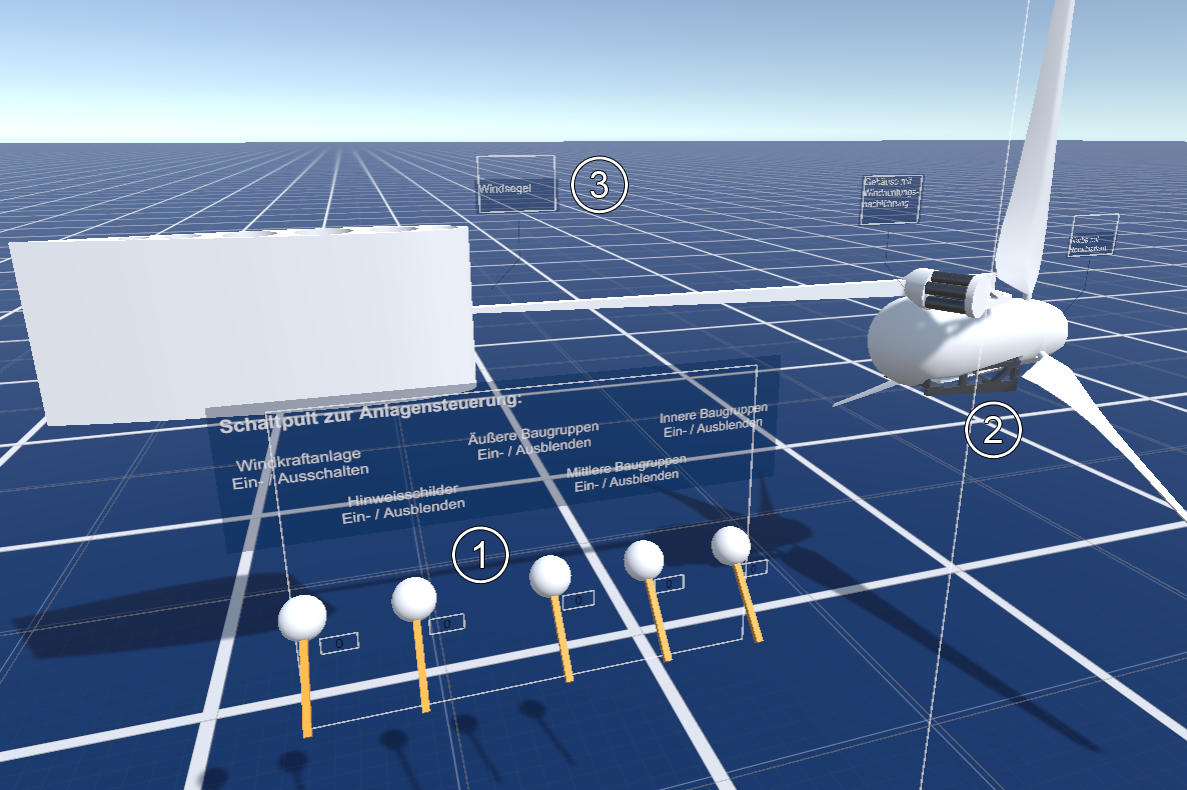
\includegraphics[keepaspectratio, width=1\textwidth]{bildquellen/szene}
	\caption{Szene in Unity.}
	\label{fig:4.1}
\end{figure}

Um die Szene zu strukturieren wurde die hierarchische Gruppierung vom VRTK-Framework übernommen. Diese der Szene untergeordneten GameObjects enthalten alle wichtigen Komponenten, welche für das Funktionieren der VR-Anwendung erforderlich sind. Die Folgende Struktur soll den hierarchischen Szenenaufbau verdeutlichen.

\begin{itemize}
\item[>] \textbf{Szene} 
	
	\begin{itemize}
	\item[>] \textbf{[VRTK\_SDKManager]:} Lädt Konfigurationen der SDKs (Windows MR, Oculus, SteamVR, UnityXR, VR-Simulator) und legt die Startreihenfolge fest.  	

		\begin{itemize}
			\item[>]\textbf{[VRTK\_SDKSetups]:} Enthält die Konfigurationsobjekte der oben genannten SDKs inklusive CameraRig, welches Kopf (Kamera) und Hände (Controller) beinhaltet.  		
		\end{itemize}
	
	\item[>] \textbf{[VRTK\_Scripts]:} Enthält obligatorische Skripte wie die Konfigurationsskripte für die Controllersteuerung.
					
	\item[>] \textbf{[SceneScripts]:} Enthält optionale Skripte wie Teleporter, AvatarHandVisibility, Bodyphysics etc.
	\item[>] \textbf{SceneObjects:} Enthält alle Szenenobjekte wie die Anlagensteuerung und die WEA.
	\end{itemize}
	
\end{itemize}


\section{Implementierte Anwendungsfälle}
\label{sec:ImplementierteAnwendungsfälle}

Im Folgenden werden die implementierten Anwendungsfälle erläutert und deren Funktionalität beschrieben.

\textbf{WEA Ein-/Ausschalten:} Der Anwendungsfall WEA Ein-/Ausschalten beschreibt die Start-/Stopp-Animation der WEA. Per Default befindet sich der Rotor der WEA in Rotation, was die Idle-Animation ist. Bei Betätigung des Schalters wird eine Brems-Animation gestartet. Im bewegungslosen Zustand wird eine Situation ohne Wind oder ein Wartungsmodus simuliert. Während der Idle-Animation erzeugt die WEA Strom.

\textbf{Hinweisschilder Ein-/Ausblenden:} Dieser Anwendungsfall beschreibt das  Ein-/Ausblenden der Hinweisschilder. Per Default sind die Hinweisschilder aktiviert. Die Funktionalität dient vor allem dazu die Übersicht zu verbessern, falls eine Betrachtung der Bauteile durch die Hinweisschilder erschwert wird. 

Der Schalter gibt, je nach Winkel einen normalisierten Float-Wert zwischen 0,0 und 1,0 zurück. Dieser Wert wird an das Skalierungsattribut der Hinweisschilder übergeben und steuert so die Größe und dementsprechend die Sichtbarkeit.  

\textbf{Baugruppen Ein-/Ausblenden:} Dieser Anwendungsfall bezieht sich auf mehrere Funktionalitäten, die das Ein- und Ausblenden von Bauteilen zur Folge haben. Dies dient dazu Innere Baugruppen der WEA sichtbar zu machen, die sonst durch äußere verdeckt sind.

Durch Betätigung des Schalters werden entsprechende Bauteile ausgefaded. Der Schalter übergibt einen normalisierten Float-Wert zwischen 0,0 und 1,0 an den Alpha-Kanal des Materials, welches dem auszublendenden Objekt zugewiesen ist. 1,0 entspricht dem Farbwert 255 (opak), 0,0 entspricht dem Farbwert 0 (volltransparent). Alle Werte zwischen 0,0 und 1,0 entsprechen Graustufen (halbtransparent). Auf diese Weise können Baugruppen ebenenweise zu- und abgeschaltet werden\sieheAbb{4.2}. 

\begin{figure}[H]
	\centering
	\captionsetup{width=1\textwidth}
	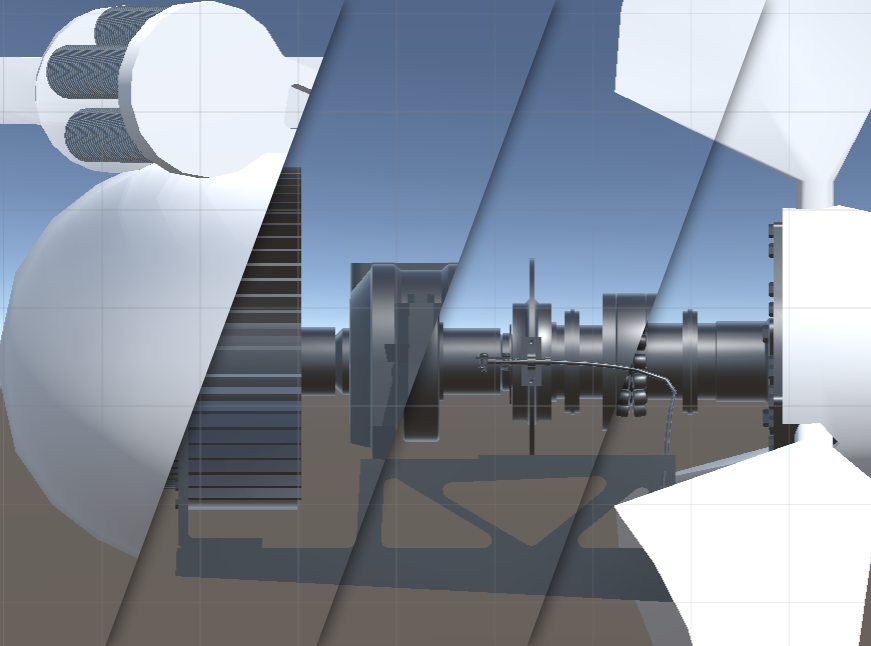
\includegraphics[keepaspectratio, width=1\textwidth]{bildquellen/baugruppen_klein}
	\caption{Zu- und abschaltbare Ebenen der WEA.}
	\label{fig:4.2}
\end{figure}


 \clearpage
\input{chapter/5fazit} \clearpage

%%Verzeichnisse
\pagenumbering{Alph}

%Literatur

\begin{thebibliography}{999}
\label{WindEnergie}
\bibitem{WindEnergie} 
Bundesverband WindEnergie e. V.  (2018): \textit{Funktionsweise von Windenergieanlagen}.\newline
\url{https://www.wind-energie.de/themen/anlagentechnik/funktionsweise/},\newline 
abgerufen am 20.08.2018.

\label{Windpumpsysteme}
\bibitem{Windpumpsysteme} 
Silvio Chemnitz, Sylvio Donner, Florian Hinze, Mats Mojem, Patrick Quandt, Oliver Seidler, Moritz Will, Jens Wuthe (2013): \textit{Windpumpsysteme zur dezentralen Energieversorgung von Abwassersystemen}. TU Berlin.

\label{Bordnetze}
\bibitem{Bordnetze}
Prof. Dr. G. Buch, Prof. Dr. M. Krug (2012): \textit{Kurzskriptum zur Lehrveranstaltung „Elektrische Bordnetze“ im Studiengang Fahrzeugtechnik}. Hochschule München.

\label{CAD}
\bibitem{CAD}
Dipl. Ing. (FH) Bettina Clauß, Helmut Prof. Dr.-Ing. von Eiff (2013):\textit{CAD Grundkurs}. Hochschule Esslingen.

\bibitem{WikiCAD}
Wikipedia  (2018): \textit{CAD}.\newline
\url{https://de.wikipedia.org/w/index.php?title=CAD&oldid=178934444},\newline 
abgerufen am 23.08.2018.


\end{thebibliography}
 \clearpage

\lstlistoflistings \relax

% Anhang


\appendix
\renewcommand\thesection{\Alph{section}}
\addchap{Anhang}

\section{Quellen}

\begin{enumerate}[label=A\arabic*]

\item \textit{Windpumpsysteme zur dezentralen Energieversorgung von Abwassersystemen} [PDF]
\item \textit{Kurzskriptum zur Lehrveranstaltung„Elektrische Bordnetze“im Studiengang Fahrzeugtechnik} [PDF]
\item \textit{CAD-Grundkurs} [PDF]
\item \textit{Vergleich von Dateiformatenfür 3D-Modelle} [PDF] 
\item \textit{STL Files and Slicing Software} [PDF] 
\end{enumerate}

\section{Software}

\begin{enumerate}[label=B\arabic*]

\item \textit{IndustrialVR Prototyp} [Unity-Anwendung]
\item \textit{IndustrialVR Projekt} [\url{https://github.com/ChrisWodaege/IndustrialVR.git}]

\end{enumerate} \clearpage

%\listoftables \clearpage

%\printindex \clearpage
%\printglossary[title={Glossar}] \clearpage
%\printglossary[style=dottedlocations,type=\acronymtype,title={Abkürzungsverzeichnis}] \clearpage
%\printbibliography[heading=bibintoc, keyword={book}, title={Literaturverzeichnis}]\clearpage
%\printbibliography[heading=bibintoc, keyword={online}, title={Onlinequellen}]\clearpage
%\printbibliography[heading=bibintoc, keyword={image}, title={Bildquellen}]\clearpage


\end{document}